\documentclass[border=4pt]{standalone}
\usepackage{amsmath, amssymb, amsfonts}
\usepackage{tikz}
% Shared TikZ style for the deep-learning computation-graph figures.
% Change notation/appearance in ONE place here and rebuild all figures.
\usetikzlibrary{arrows.meta, positioning, calc}

% Colours for forward-pass / backprop highlights
\definecolor{fwdblue}{RGB}{0,0,255}
\definecolor{bpred}{RGB}{255,0,0}

\tikzset{
    % filled dot used for inputs, biases and indicator vectors
    unit/.style={circle, fill=black, inner sep=0pt, minimum size=5pt},
    % linear transformation node (weighted sum), drawn as a circled plus
    sumop/.style={circle, draw, thick, inner sep=1pt, minimum size=16pt},
    % non-linear transformation, a labelled box with vertical text
    opbox/.style={draw, thick, minimum width=22pt, inner sep=6pt},
    % directed edges
    edge/.style={-{Latex[length=6pt]}, thick},
    % edge labels (variable names on the wires)
    wire/.style={font=\normalsize, inner sep=2pt},
}

% vertical text for the operation boxes
\newcommand{\vlabel}[1]{\rotatebox{90}{#1}}


\begin{document}
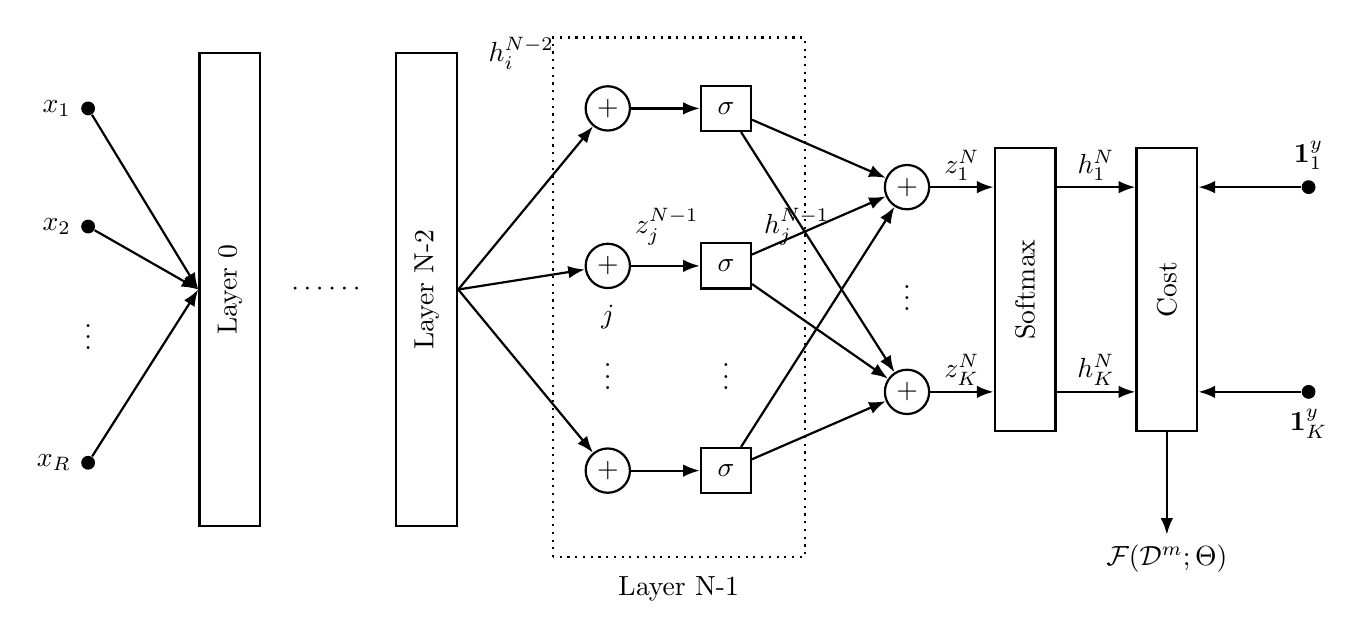
\begin{tikzpicture}[>=Latex]

    % ---- inputs ----
    \node[unit, label=left:{$x_1$}] (x1) at (0, 3)    {};
    \node[unit, label=left:{$x_2$}] (x2) at (0, 1.5)  {};
    \node                            (xd) at (0, 0.2)  {$\vdots$};
    \node[unit, label=left:{$x_R$}] (xR) at (0, -1.5) {};

    % ---- layer boxes ----
    \node[opbox, minimum height=6cm] (L0) at (1.8, 0.7) {\vlabel{Layer 0}};
    \node at (3.05, 0.7) {$\cdots\cdots$};
    \node[opbox, minimum height=6cm] (L2) at (4.3, 0.7) {\vlabel{Layer N-2}};

    \foreach \x in {x1,x2,xR}{ \draw[edge] (\x) -- (L0.west); }

    % ---- hidden layer N-1 : sum + sigma ----
    \node[sumop] (hA) at (6.6, 3)    {$+$};
    \node[sumop] (hB) at (6.6, 1)    {$+$};
    \node        (hd) at (6.6, -0.3) {$\vdots$};
    \node[sumop] (hC) at (6.6, -1.6) {$+$};

    \node[opbox, minimum size=16pt] (gA) at (8.1, 3)    {$\sigma$};
    \node[opbox, minimum size=16pt] (gB) at (8.1, 1)    {$\sigma$};
    \node                            (gd) at (8.1, -0.3) {$\vdots$};
    \node[opbox, minimum size=16pt] (gC) at (8.1, -1.6) {$\sigma$};

    % Layer N-2 -> hidden sums (fan out)
    \foreach \h in {hA,hB,hC}{ \draw[edge] (L2.east) -- (\h); }
    % sum -> sigma
    \foreach \h/\g in {hA/gA,hB/gB,hC/gC}{ \draw[edge] (\h) -- (\g); }

    % ---- final linear layer ----
    \node[sumop] (fA) at (10.4, 2)    {$+$};
    \node        (fd) at (10.4, 0.7)  {$\vdots$};
    \node[sumop] (fB) at (10.4, -0.6) {$+$};

    % sigma -> final sums (fan out)
    \foreach \g in {gA,gB,gC}{
        \draw[edge] (\g) -- (fA);
        \draw[edge] (\g) -- (fB);
    }

    % ---- softmax / cost ----
    \node[opbox, minimum height=3.6cm] (soft) at (11.9, 0.7) {\vlabel{Softmax}};
    \node[opbox, minimum height=3.6cm] (cost) at (13.7, 0.7) {\vlabel{Cost}};

    \draw[edge] (fA) -- (soft.west |- fA) node[wire, midway, above] {$z_1^N$};
    \draw[edge] (fB) -- (soft.west |- fB) node[wire, midway, above] {$z_K^N$};
    \draw[edge] (soft.east |- fA) -- (cost.west |- fA)
        node[wire, midway, above] {$h_1^N$};
    \draw[edge] (soft.east |- fB) -- (cost.west |- fB)
        node[wire, midway, above] {$h_K^N$};

    % indicators
    \node[unit, label=above:{$\mathbf{1}^y_1$}] (i1) at (15.5, 2)    {};
    \node[unit, label=below:{$\mathbf{1}^y_K$}] (iK) at (15.5, -0.6) {};
    \draw[edge] (i1) -- (cost.east |- fA);
    \draw[edge] (iK) -- (cost.east |- fB);

    \draw[edge] (cost.south) -- ++(0, -1.3)
        node[below] {$\mathcal{F}(\mathcal{D}^m; \Theta)$};

    % ---- annotations ----
    \node at (5.5, 3.7) {$h_i^{N-2}$};
    \node at (7.35, 1.5) {$z_j^{N-1}$};
    \node at (9.0, 1.5) {$h_j^{N-1}$};
    \node at (6.6, 0.35) {$j$};

    % dotted grouping box for layer N-1
    \draw[dotted, thick] (5.9, -2.7) rectangle (9.1, 3.9);
    \node at (7.5, -3.1) {Layer N-1};

\end{tikzpicture}
\end{document}
